\documentclass[11pt,a4paper]{article}
\usepackage[T1]{fontenc}
\usepackage[margin=2.3cm]{geometry}
\usepackage{amsmath,amssymb}
\usepackage{graphicx}
\usepackage[dvipsnames]{xcolor}
\usepackage{enumitem}
\usepackage[colorlinks=true,linkcolor=blue,urlcolor=blue]{hyperref}
\setlength{\parskip}{0.6em}
\setlength{\parindent}{0pt}
\begin{document}

\begin{center}{\LARGE\bfseries opengears}\\[0.4em]{\large Design a gearbox train to hit a target ratio and torque, in three sessions.}\\[0.2em]\small PAN IIT OSS explainer \textbullet{} diploma / undergraduate to advanced undergraduate (levels 5-6)\end{center}

\section*{Why this exists}
Every gearbox is a promise: more torque for less speed, from a few whole numbers of teeth. This explainer shows the mathematics behind gear trains, ratios, losses and backlash, so you can design one yourself.

\section*{The end goal}
Design a gearbox train to hit a target ratio and torque. The end goal is designing a gearbox train to hit a target ratio and torque: choosing tooth counts that give the ratio, fit the box, avoid undercutting and survive start-up. The same ideas size the drives of winches, robots and vehicles.

\section*{How the three sessions build up}
\begin{enumerate}[nosep]
\item \textbf{Session 1: Two gears trade speed for torque} (Level 1, conceptual interactive model, 60 min).
\item \textbf{Session 2: Compound trains, module and a 1:20 design} (Level 2, mathematical engineering model, 75 min).
\item \textbf{Session 3: Search, losses, backlash and a planetary set} (Level 3, simulation and validation, 90 min).
\end{enumerate}

\section{Session 1: Two gears trade speed for torque}

\subsection*{A. Real-world problem}
A bicycle chain, a hand drill and the gearbox of a car all do one trick: they make a motor or a leg turn at a different speed with a different twisting force. You push a small gear and it turns a big gear slowly, but the big gear can lift much more. How is the speed given up and the strength gained, which way does each gear turn, and what does a gear in the middle (an idler) do?

\subsection*{B. Concept and theory}
Two gears mesh when their teeth fit together, so as one turns the teeth pass the contact point one after another: the same number of teeth pass on both gears. If the driving gear (the driver) has N\_driver teeth and turns at w\_in, N\_driver w\_in teeth pass per minute, and the driven gear must turn at w\_out = w\_in N\_driver / N\_driven. The speed ratio is i = N\_driven / N\_driver; i greater than 1 is a reduction. An ideal gear loses no energy, so power P = T w is the same on both sides, which means the torque goes up by the same factor: T\_out = T\_in i. External gears turn in opposite directions, so in a row of gears with k meshes the last gear turns the same way as the first only if k is even. A gear in the middle of the row (an idler) cancels out of the ratio but still adds a mesh, so it flips the direction.

\begin{itemize}[nosep]
\item N\_driver, N\_driven: number of teeth on the driving and the driven gear (teeth)
\item w: rotation speed (rpm (revolutions per minute))
\item T: torque (twisting force times arm length) (N m)
\item i: speed ratio N\_driven / N\_driver (no unit)
\item k: number of meshes in the train (no unit)
\item P: power, torque times angular speed in rad/s (W)
\end{itemize}

\begin{equation*}
i=\frac{N_\mathrm{driven}}{N_\mathrm{driver}}
\end{equation*}

\begin{equation*}
\omega_\mathrm{out}=\frac{\omega_\mathrm{in}}{i},\qquad T_\mathrm{out}=i\,T_\mathrm{in}\quad\text{(ideal)}
\end{equation*}

\begin{equation*}
P=T\,\omega,\qquad \omega=\frac{2\pi n}{60}\quad(n\text{ in rpm},\ \omega\text{ in rad/s})
\end{equation*}

\begin{equation*}
\text{direction after }k\text{ meshes}=(-1)^k
\end{equation*}

\begin{center}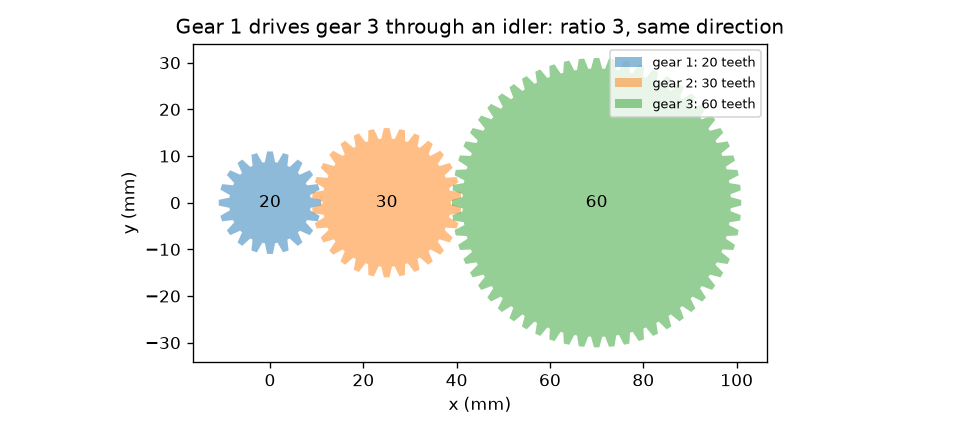
\includegraphics[width=0.85\linewidth]{figures/s01_gear_train.png}\\\small A 20-tooth gear drives a 60-tooth gear through a 30-tooth idler: ratio 3, same direction.\end{center}

\subsection*{E. Worked example}
A 20-tooth gear turns at 120 rpm with 5 N m and drives a 60-tooth gear. Find the output speed, torque and direction, and check the power. Then put a 30-tooth idler between them.
\begin{enumerate}[nosep]
\item Ratio i = 60 / 20 = 3.
\item Output speed = 120 / 3 = 40 rpm, and the direction is opposite (one mesh).
\item Ideal output torque = 5 * 3 = 15 N m.
\item Power in = 5 N m * 120 rpm * 2 pi / 60 = 5 * 12.566 = 62.83 W. Power out = 15 * 4.189 = 62.83 W. They agree.
\item With the 30-tooth idler there are two meshes: the output is 40 rpm and 15 N m again, now in the same direction as the input.
\end{enumerate}
\textbf{Answer.} 40 rpm and 15 N m opposite to the input (62.83 W both sides); with an idler, the same 40 rpm and 15 N m in the same direction.

\subsection*{F. Questions}
\begin{enumerate}[nosep]
\item \textbf{Conceptual.} If the driven gear has twice as many teeth as the driving gear, what is the ideal output speed ratio, and what real-world losses should be considered?
\item \textbf{Numerical.} A 40-tooth gear drives a 20-tooth gear at 100 rpm and 4 N m. Find the output speed and ideal torque, and say what kind of train this is.
\item \textbf{Graph and simulation interpretation.} In the speed and torque graphs for a 20-tooth driver at 120 rpm and 5 N m, read the output speed and torque when the driven gear has 40 teeth and when it has 60 teeth. What happens to their product?
\item \textbf{Design and optimisation challenge.} Design: from a 20-tooth driver at 120 rpm and 5 N m you need 40 rpm out turning the same way as the input. Choose the driven gear and the idlers, and state the output torque. What is the price of an idler?
\end{enumerate}

\section{Session 2: Compound trains, module and a 1:20 design}

\subsection*{A. Real-world problem}
A motor turns at 1200 rpm and a conveyor must turn at 60 rpm: a 1:20 reduction. One pair of gears would need a 17-tooth pinion and a 340-tooth gear, which at module 2 mm would be 680 mm across. Real gearboxes use two stages instead. Which tooth counts give exactly 1:20, with no pinion so small that its teeth are cut away, and the smallest gears?

\subsection*{B. Concept and theory}
In a compound train two gears sit on the same shaft and turn together; the first stage is N1 driving N2, the second is N3 (on the N2 shaft) driving N4. The stage ratios multiply: i = (N2 / N1)(N4 / N3). Output speed is w\_in / i and the ideal output torque is T\_in i, so power is unchanged. Every external mesh flips the direction, so two meshes turn the output the same way as the input. Gears that mesh must share the module m (tooth size in mm); a gear with N teeth has pitch diameter d = m N, and two meshing gears sit a centre distance a = (d1 + d2) / 2 = m (N1 + N2) / 2 apart. Gear cutting can remove the root of a tooth of a small pinion (undercutting); for a 20 degree pressure angle the geometric limit is 2 / sin\textasciicircum{}2(20 degrees) = 17.1 teeth, so 17 teeth is a commonly used practical guideline. The contact ratio (the average number of tooth pairs in contact) must be above 1 so that the load passes smoothly from tooth to tooth.

\begin{itemize}[nosep]
\item N1..N4: tooth counts of gears 1 to 4 (teeth)
\item i: overall speed ratio (no unit)
\item m: module (tooth size) (mm)
\item d: pitch diameter m N (mm)
\item a: centre distance of a mesh (mm)
\item phi: pressure angle (20 degrees is standard) (degrees)
\item w, T: speed and torque (rpm, N m)
\end{itemize}

\begin{equation*}
i=\frac{N_2}{N_1}\cdot\frac{N_4}{N_3},\qquad \omega_\mathrm{out}=\frac{\omega_\mathrm{in}}{i},\qquad T_\mathrm{out}=i\,T_\mathrm{in}
\end{equation*}

\begin{equation*}
d=mN,\qquad a=\frac{d_1+d_2}{2}=\frac{m(N_1+N_2)}{2}
\end{equation*}

\begin{equation*}
N_\mathrm{min}=\frac{2}{\sin^2\varphi}\approx 17.1\quad(\varphi=20^\circ)
\end{equation*}

\begin{equation*}
\varepsilon=\frac{\sqrt{r_{a1}^2-r_{b1}^2}+\sqrt{r_{a2}^2-r_{b2}^2}-a\sin\varphi}{\pi m\cos\varphi}
\end{equation*}

\begin{center}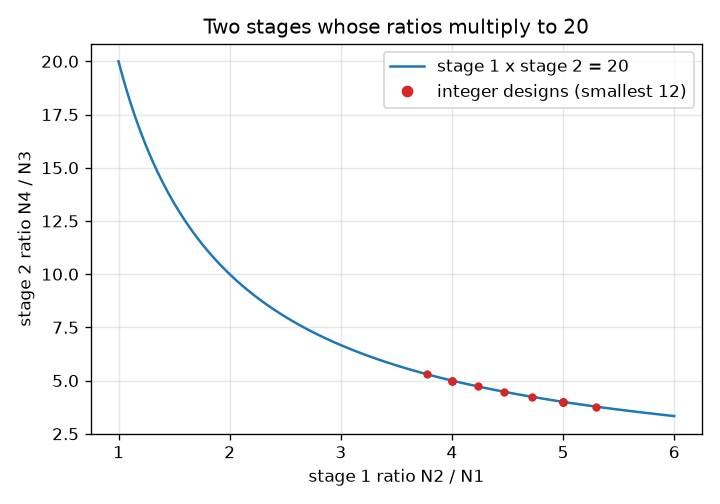
\includegraphics[width=0.85\linewidth]{figures/s02_ratio_hyperbola.png}\\\small All pairs of stage ratios with product 20 (blue) and the smallest integer designs (red).\end{center}

\subsection*{E. Worked example}
Reduce 1200 rpm to 60 rpm (ratio 20) with two stages, whole numbers of teeth from 17 to 100, and the fewest total teeth. Give the speeds and ideal torques for a 2 N m input, and check the centre distances at module 2 mm.
\begin{enumerate}[nosep]
\item We need (N2 / N1)(N4 / N3) = 20. List every pair (N\_driver, N\_driven) with 17 to 100 teeth, group them by exact ratio, and join two groups whose ratios multiply to 20: there are 146 such designs (counting both orders).
\item The smallest total is 17 + 68 + 17 + 85 = 187 teeth: stage ratios 68 / 17 = 4 and 85 / 17 = 5, and 4 * 5 = 20 exactly.
\item Speeds: 1200 / 4 = 300 rpm on the middle shaft (reversed), then 300 / 5 = 60 rpm on the output (same way as the input).
\item Ideal torques: 2 N m, then 2 * 4 = 8 N m, then 8 * 5 = 40 N m. The power is the same on every shaft.
\item Centre distances at module 2 mm: 2 * (17 + 68) / 2 = 85 mm and 2 * (17 + 85) / 2 = 102 mm. They are not equal, so the output shaft is not in line with the input shaft (only 4 of the 146 designs are in line; Session 3 searches for them).
\end{enumerate}
\textbf{Answer.} 17-68 then 17-85 (187 teeth): 1200 to 300 to 60 rpm, 2 to 8 to 40 N m ideal, same direction as the input, but the centre distances are 85 mm and 102 mm.

\subsection*{F. Questions}
\begin{enumerate}[nosep]
\item \textbf{Conceptual.} Why is a two-stage train better than one pair of gears for a 1:20 reduction? Give two reasons.
\item \textbf{Numerical.} A train has stages 20-50 and 18-72. Find the overall ratio, the output speed and the ideal output torque for 900 rpm and 3 N m in, and the direction.
\item \textbf{Graph and simulation interpretation.} In the ratio graph with N1 = 20, N2 = 60 and N3 = 20, which N4 gives a ratio of 20? Can you set that on the slider?
\item \textbf{Design and optimisation challenge.} Design: find the exact two-stage reduction of 1:12 with 17 to 100 teeth and the fewest total teeth. Give the centre distances at module 2 mm.
\end{enumerate}

\section{Session 3: Search, losses, backlash and a planetary set}

\subsection*{A. Real-world problem}
The smallest 1:20 design of Session 2 had centre distances of 85 mm and 102 mm, so a gearbox with the input and output shafts in line cannot be built from it. A real design must also hit the ratio to a tolerance, survive a torque pulse when the motor starts, and waste little power. Which tooth counts work, what do 2 percent per mesh and a loose fit between the teeth cost, and how does a planetary gear set pack a large ratio into a small space?

\subsection*{B. Concept and theory}
Search: for two stages with the same module the shafts are in line when N1 + N2 = N3 + N4. Numpy tests every (N2, N3, N4) for each N1 at once. Losses: each mesh transmits about 98 percent of the power (a typical figure; real values depend on gears, lubricant and load), so n meshes keep 0.98\textasciicircum{}n, and power in = power out + loss. Dynamics: refer every shaft to the input by dividing its angle by its ideal ratio rho; its inertia then counts as J rho\textasciicircum{}2, and a mesh is a spring k with a dead zone b (backlash) and damping c while the teeth touch. When all teeth touch, the train acts as one inertia J\_eff = sum of J rho\textasciicircum{}2 (for one stage J1 + J2 (N1 / N2)\textasciicircum{}2). Two exact checks: the total momentum sum J rho\textasciicircum{}2 w grows by exactly the torque impulse (internal mesh forces cancel), and input work = kinetic energy + spring energy + energy lost in damping. Planetary set: a sun (Ns teeth), a ring (Nr teeth, internal) and planets on a carrier (Np = (Nr - Ns) / 2 teeth). The Willis relation w\_sun Ns + w\_ring Nr = w\_carrier (Ns + Nr) links the three speeds; with the ring fixed and the sun as input the ratio is 1 + Nr / Ns. The planets must also space evenly: (Ns + Nr) must be divisible by the number of planets.

\begin{itemize}[nosep]
\item N1..N4: tooth counts (teeth)
\item tol: allowed relative ratio error (no unit)
\item eta: efficiency per mesh (typical 0.98) (no unit)
\item rho: ideal speed of a shaft divided by the input speed (no unit)
\item J: shaft inertia (kg m\textasciicircum{}2)
\item k, c, b: mesh stiffness, damping and backlash, referred to the input (N m/rad, N m s/rad, rad)
\item w\_sun, w\_ring, w\_carrier: speeds of the planetary set (rpm)
\item Ns, Nr: sun and ring teeth (teeth)
\end{itemize}

\begin{equation*}
\varepsilon=\left|\frac{N_2N_4}{N_1N_3\,i_\mathrm{target}}-1\right|\le \mathrm{tol},\qquad N_1+N_2=N_3+N_4\ \text{(in line)}
\end{equation*}

\begin{equation*}
\eta_\mathrm{total}=\eta^{\,n},\qquad P_\mathrm{in}=P_\mathrm{out}+P_\mathrm{loss}
\end{equation*}

\begin{equation*}
J_\mathrm{eff}=\sum_i J_i\rho_i^{2}=J_1+J_2\Big(\frac{N_1}{N_2}\Big)^{2}+\dots
\end{equation*}

\begin{equation*}
\sum_i J_i\rho_i^{2}\,\dot\varphi_i=\int T\,dt,\qquad \int T\dot\varphi_1\,dt=E_\mathrm{kin}+E_\mathrm{spring}+E_\mathrm{lost}
\end{equation*}

\begin{equation*}
\omega_s N_s+\omega_r N_r=\omega_c\,(N_s+N_r),\qquad \frac{\omega_s}{\omega_c}=1+\frac{N_r}{N_s}\ \ (\omega_r=0)
\end{equation*}

\begin{center}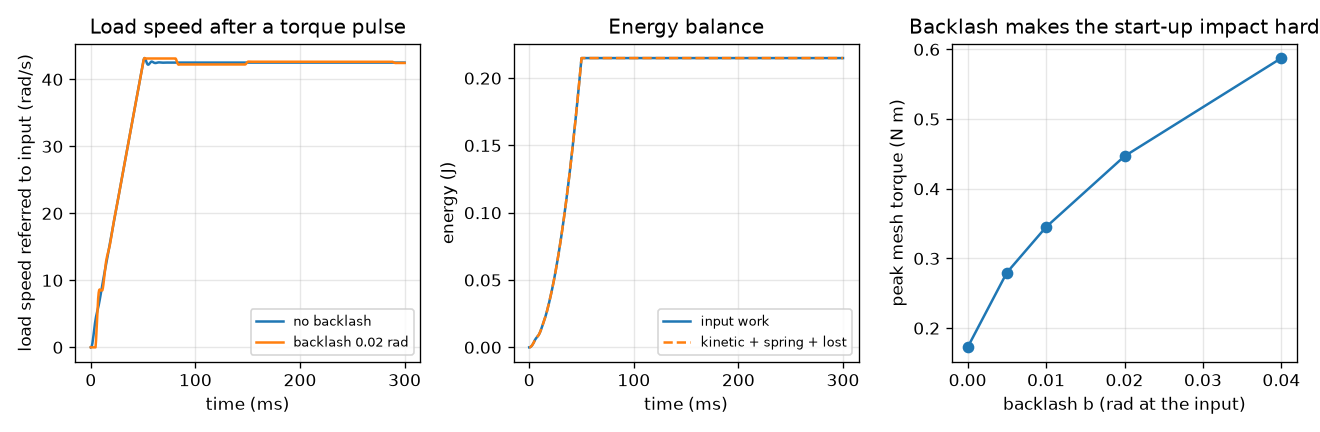
\includegraphics[width=0.85\linewidth]{figures/s03_dynamics.png}\\\small Torque pulse on a two-stage train: speeds, energy balance and the peak mesh torque against backlash.\end{center}

\subsection*{E. Worked example}
Search 17 to 90 teeth for an in-line two-stage 1:20 within 1 percent and take the design with the fewest teeth. Then, for input and load inertias J1 = 1e-4, middle shaft 2e-4 and load 0.05 kg m\textasciicircum{}2, find J\_eff, the input speed after a 0.2 N m pulse of 0.05 s, and the output speed.
\begin{enumerate}[nosep]
\item No exact in-line 1:20 exists in this range, but 19 designs lie within 1 percent; the fewest teeth are in 17-76 then 17-76 with ratio (76 / 17)\textasciicircum{}2 = 19.986.
\item Both stages have N + N = 93, so the centre distances are equal and the shafts are in line.
\item rho for the shafts: 1, 17 / 76 = 0.2237, and 0.2237\textasciicircum{}2 = 0.0500.
\item J\_eff = 1e-4 + 2e-4 * 0.0500 + 0.05 * 0.0500\textasciicircum{}2 = 1.0e-4 + 1.0e-5 + 1.25e-4 = 2.352e-4 kg m\textasciicircum{}2.
\item Impulse = 0.2 * 0.05 = 0.01 N m s, so the input turns at 0.01 / 2.352e-4 = 42.5 rad/s once the teeth are all in contact (the simulation gives 42.5).
\item Output speed = 42.5 * 0.0500 = 2.13 rad/s = 20.3 rpm. At 98 percent per mesh, 2 meshes would keep 0.9604 of the power.
\end{enumerate}
\textbf{Answer.} 17-76-17-76 (ratio 19.986, 93 + 93 in line); J\_eff = 2.352e-4 kg m\textasciicircum{}2; the input reaches 42.5 rad/s and the output 20.3 rpm. The simulation agrees: momentum equals the impulse and input work equals kinetic + spring + lost energy.

\subsection*{F. Questions}
\begin{enumerate}[nosep]
\item \textbf{Conceptual.} Why does backlash make the start-up impact harder, and why is the final speed hardly affected?
\item \textbf{Numerical.} A planetary set has Ns = 24 and Nr = 72. With the ring fixed and the sun at 900 rpm, find the planet teeth, the ratio and the carrier speed. Then a four-mesh spur train takes 500 W: how much power is lost at 98 percent per mesh?
\item \textbf{Graph and simulation interpretation.} In the mesh-torque view, the peak mesh torque is 0.172 N m for no backlash and 0.447 N m for 0.02 rad. At 0.04 rad it is 0.588 N m. What is the trend and what does it mean for gear wear?
\item \textbf{Design and optimisation challenge.} Design: find the in-line two-stage gearbox for 1:16 within 1 percent with 17 to 90 teeth and the fewest total teeth. Is the ratio exact? Check it with the checker at module 2 mm.
\end{enumerate}

\section{Real-world mini-project}
\textbf{Choose a gear train for a hand-crank winch.} A hand-crank winch must hold and lift a 50 kg load on a rope drum of radius 0.12 m, using a crank of radius 0.15 m, 40 rpm at the crank and a rope speed of at least 0.10 m/s. The hand force must stay at or below 85 N (a 15 percent margin under the 100 N limit), each mesh gets 98 percent (typical), the gears are module 2 mm, and every mesh must stay within an 80 mm centre distance. Use \texttt{crank\_force}, \texttt{rope\_speed} and \texttt{winch\_candidates} from Session 3 (illustrative numbers, not a real design). Show that no single stage works, then pick a two-stage train with an engineering argument.

\section{The path ahead}
\begin{enumerate}[nosep]
\item \textbf{Session 4: Helical gears and a smoother mesh.} A contact-ratio function for helical gears and a comparison with spur gears.
\item \textbf{Session 5: Three stages in line.} A grouped search for in-line three-stage trains.
\item \textbf{Session 6: Two planetary stages in series.} A designer that picks Ns, Nr and the planet count for each stage.
\item \textbf{Session 7: Worm drives and self-locking.} A worm-pair model with efficiency and a self-locking test.
\item \textbf{Session 8: Torsional resonance of the train.} An eigenvalue calculation for the mesh-spring model.
\end{enumerate}

\section{Answers and hints}

\subsection*{Session 1}
\begin{enumerate}[nosep]
\item \textbf{Conceptual.} Hint: Teeth passing the contact point are equal on both gears. Then think about what rubs, slips or churns in a real gearbox. Solution: The driven gear turns at half the input speed (the speed ratio i = 2, a reduction) and, ideally, delivers twice the torque, in the opposite direction. In a real gearbox the output torque is a little less than twice because of friction between sliding teeth, bearing and seal friction, oil churning, and wasted motion across the backlash. These losses turn some input power into heat.
\item \textbf{Numerical.} Hint: i = N\_driven / N\_driver = 20 / 40. Solution: i = 20 / 40 = 0.5, so the speed goes up: 100 / 0.5 = 200 rpm (opposite direction). Ideal torque = 4 * 0.5 = 2 N m. This is a speed-up (overdrive): the output is faster and weaker. Power check: 4 * 10.47 = 41.9 W = 2 * 20.94 = 41.9 W.
\item \textbf{Graph and simulation interpretation.} Hint: Use speed = 120 * 20 / N and torque = 5 * N / 20. Solution: At 40 teeth: 60 rpm and 10 N m. At 60 teeth: 40 rpm and 15 N m. Speed falls and torque rises. The product of torque and speed (proportional to power) stays the same: 10 * 60 = 600 and 15 * 40 = 600 in these units, so the power is unchanged.
\item \textbf{Design and optimisation challenge.} Hint: You need ratio 3 and an even number of meshes. Solution: Driven gear with 60 teeth (ratio 3). Two meshes means one idler (any tooth count, for example 30; it does not change the ratio). Output: 40 rpm and 15 N m ideal, same direction. The price of an idler is one more mesh: more friction loss, more parts and more space. Session 3 puts a number on the loss.
\end{enumerate}

\subsection*{Session 2}
\begin{enumerate}[nosep]
\item \textbf{Conceptual.} Hint: Compare the biggest gear in each design, at module 2 mm. Solution: One stage with the 17-tooth pinion needs a 340-tooth gear, a pitch diameter of 2 * 340 = 680 mm. The two-stage design's biggest gear has 85 teeth, 2 * 85 = 170 mm across: smaller, lighter and cheaper to make, and it fits in a smaller housing. Also each pair keeps a moderate ratio (4 and 5), which keeps tooth sizes and loads reasonable.
\item \textbf{Numerical.} Hint: Multiply the stage ratios. Solution: i = (50 / 20)(72 / 18) = 2.5 * 4 = 10. Output speed = 900 / 10 = 90 rpm. Ideal output torque = 3 * 10 = 30 N m. Two meshes, so the output turns the same way as the input. Power check: the torque rose 10 times and the speed fell 10 times.
\item \textbf{Graph and simulation interpretation.} Hint: The ratio is N2 N4 / (N1 N3), a straight line in N4. Solution: The line is ratio = 60 * N4 / 400 = 0.15 N4. Setting it to 20 gives N4 = 133.3, which is outside the slider range (30 to 100) and not a whole number. The line is below 20 everywhere on the graph; you have to change N1, N2 or N3 too.
\item \textbf{Design and optimisation challenge.} Hint: Try stage ratios such as 3 and 4, and the pinion 17. Solution: 17-51 (ratio 3) then 17-68 (ratio 4): 3 * 4 = 12, total 17 + 51 + 17 + 68 = 153 teeth. Centre distances at module 2 mm: 2 * (17 + 51) / 2 = 68 mm and 2 * (17 + 68) / 2 = 85 mm: not equal, so the shafts are not in line. Trade-off: the smallest design is not always the one that fits the housing.
\end{enumerate}

\subsection*{Session 3}
\begin{enumerate}[nosep]
\item \textbf{Conceptual.} Hint: Think about what the motor side does while the teeth are not touching, and what is conserved. Solution: While the gap closes the motor side accelerates alone with only part of the inertia, so it hits the load side at a higher relative speed and the mesh torque spikes. The momentum is conserved (internal mesh forces cancel), so once the oscillation dies the speeds settle to nearly the same values: backlash changes the shock and the delay, not the final speed.
\item \textbf{Numerical.} Hint: Np = (Nr - Ns) / 2 and ratio = 1 + Nr / Ns; 0.98\textasciicircum{}4. Solution: Np = (72 - 24) / 2 = 24 teeth. Ratio = 1 + 72 / 24 = 4, so the carrier turns at 900 / 4 = 225 rpm (Willis: 900 * 24 = w\_c * 96). For the spur train: 0.98\textasciicircum{}4 = 0.9224, so 500 * 0.9224 = 461.2 W comes out and 38.8 W is lost.
\item \textbf{Graph and simulation interpretation.} Hint: Compare the three values and ask what a bigger gap does to the impact. Solution: The peak rises with backlash: 0.172, 0.447 and 0.588 N m (and 0.345 at 0.01 rad). Even though the gap is small, a loose train takes up the gap with an impact, so tooth contact stresses and noise grow. This is why precision drives use low backlash or anti-backlash gears, at the price of more friction and cost.
\item \textbf{Design and optimisation challenge.} Hint: Use search\_trains(16, 0.01) and take the row with the smallest sum. Solution: There are 46 in-line designs; the smallest is 17-68-17-68, ratio exactly 16, both stages with N + N = 85 (centre distance 85 mm at module 2). check\_design returns no problems. Trade-off: equal stages are easy to build and in line, but two 68-tooth gears are not the smallest possible if you drop the in-line condition.
\end{enumerate}

\section{How to join}
Read \texttt{CONTRIBUTING.md} in the repository, then pick an issue labelled \texttt{good first issue}. Repository: \url{https://github.com/KrunalPanchal1995/opengears}

\end{document}
